\documentclass{beamer}

\usepackage[utf8]{inputenc}
\usepackage[T2A]{fontenc}
\usepackage[russian]{babel}

\usetheme{Madrid}
\usecolortheme{default}

\usepackage{hyperref}
\hypersetup{
    colorlinks=true,
    linkcolor=blue,
    urlcolor=blue,
}

\usepackage{listings}
\usepackage{color}
\usepackage{caption}

\definecolor{codegreen}{rgb}{0,0.6,0}
\definecolor{codegray}{rgb}{0.5,0.5,0.5}
\definecolor{codeblue}{rgb}{0,0,0.8}
\definecolor{backcolour}{rgb}{0.95,0.95,0.92}

\lstdefinestyle{mystyle}{
    backgroundcolor=\color{backcolour},
    commentstyle=\color{codegreen},
    keywordstyle=\color{codeblue},
    numberstyle=\tiny\color{codegray},
    stringstyle=\color{codegreen},
    basicstyle=\ttfamily\footnotesize,
    breakatwhitespace=false,
    breaklines=true,
    captionpos=b,
    keepspaces=true,
    numbers=left,
    numbersep=5pt,
    showspaces=false,
    showstringspaces=false,
    showtabs=false,
    tabsize=2
}
\lstset{style=mystyle}


\title{Современные методы машинного обучения}
\author{Степанова Анна}
\institute{РГПУ им. А. И. Герцена}


\begin{document}

\begin{frame}
    \titlepage
\end{frame}

\begin{frame}{Содержание}
    \tableofcontents
\end{frame}

\section{Введение}

\begin{frame}{Введение}
    \begin{block}{Актуальность}
        Машинное обучение является одной из ключевых областей искусственного интеллекта.
    \end{block}
    
    \begin{itemize}
        \item<1-> Обучение на основе данных
        \item<2-> Автоматическое выявление закономерностей
        \item<3-> Применение в различных сферах
    \end{itemize}
\end{frame}

\section{Методы}

\begin{frame}{Основные методы}
    \begin{columns}[T]
        \column{0.5\textwidth}
        \textbf{Обучение с учителем}
        \begin{itemize}
            \item Классификация
            \item Регрессия
        \end{itemize}
        
        \column{0.5\textwidth}
        \textbf{Обучение без учителя}
        \begin{itemize}
            \item Кластеризация
            \item Снижение размерности
        \end{itemize}
    \end{columns}
\end{frame}

\section{Пример кода}

\begin{frame}[fragile]{Пример кода на Python}
    \begin{lstlisting}[language=Python, caption=Обучение модели]
import numpy as np
from sklearn.ensemble import RandomForestClassifier

# Создание модели
model = RandomForestClassifier(n_estimators=100)

# Обучение
model.fit(X_train, y_train)

# Предсказание
predictions = model.predict(X_test)
    \end{lstlisting}
\end{frame}

\section{Результаты}

\begin{frame}{Результаты экспериментов}
    \begin{center}
        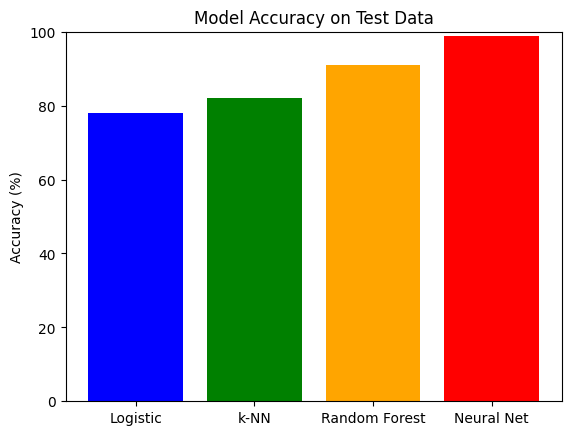
\includegraphics[width=0.6\textwidth]{graph.png}
        
        \small{График точности модели}
    \end{center}
\end{frame}

\section{Источники}

\begin{frame}{Полезные ресурсы}
    \begin{itemize}
        \item \href{https://scikit-learn.org}{Scikit-learn}
        \item \href{https://www.tensorflow.org}{TensorFlow}
        \item \href{https://pytorch.org}{PyTorch}
    \end{itemize}
\end{frame}

\section{Заключение}

\begin{frame}{Заключение}
    \begin{block}{Выводы}
        \begin{enumerate}
            \item Машинное обучение активно развивается
            \item Существует множество методов для разных задач
            \item Важно правильно выбирать модель
        \end{enumerate}
    \end{block}
\end{frame}

\begin{frame}{Спасибо за внимание!}
    \begin{center}
        \Huge \textbf{Спасибо!}
        
        \vspace{1cm}
        \Large \href{mailto:st.ann0@yandex.ru}{st.ann0@yandex.ru}
    \end{center}
\end{frame}

\end{document}
